% scopiazzato dal template di Matteo Longeri (grazie!)
%%%%%%%%%%%%%%%%%%%%%%%%%%%%%%%%%%%%%%%%%%%%%%%%%%%%%%
\documentclass[a4paper]{report}
% o article, book, ...



%%%%%%%%%%%%%%%%%%%%%%%%%%%%%%%%%%%%%%%%%%%%%%%%%%%%%%
% packages...
\usepackage[utf8]{inputenc}
\usepackage[english,italian]{babel}
\usepackage[hyphens]{url}

% Per generare il file PDF aderente alle specifiche PDF/A-1b. Verificarne poi la validità.
%\usepackage[a-1b]{pdfx}

\usepackage{hyperref}
\usepackage{graphicx}


%%%%%%%%%%%%%%%%%%%%%%%%%%%%%%%%%%%%%%%%%%%%%%%%%%%%%
\begin{document}

% Frontespizio
\begin{titlepage}
\begin{center}
\includegraphics[width=\textwidth]{Logo.jpg}\\
{\large{\bf Corso di Laurea Triennale in Informatica}}
\end{center}
\vspace{12mm}
\begin{center}
{\huge{\bf Studio sull'incidentalità stradale}}\\
\vspace{4mm}
{\huge{\bf tramite dataset aperti}}\\
\end{center}
\vspace{12mm}
\begin{flushright}
{\large{\bf Tesi di Laurea di:}}\\
{\large{\bf Gabriele Padovani}}\\
{\large{\bf Matr. 909165}}\\
\end{flushright}
\vspace{4mm}
\begin{flushleft}
{\large{\bf Relatore:}}\\
{\large{\bf Andrea Trentini}}\\
\vspace{4mm}
{\large{\bf Correlatore:}}\\
{\large{\bf CORREL}}\\
\end{flushleft}
\vspace{12mm}
\begin{center}
{\large{\bf Anno Accademico 2020/2021}}
\end{center}
\end{titlepage}


\tableofcontents

%%%%%%%%%%%%%%%%%%%%%%%%%%%%%%%%%%%%%%%%%%%%%%%%%%%%%%
\chapter{Introduzione}
% Non Ho idea di come si debba introdurre la tesi... :|

% o sections (dipende dal documentclass)
%%%%%%%%%%%%%%%%%%%%%%%%%%%%%%%%%%%%%%%%%%%%%%%%%%%%%%
\chapter{Dati Geolocalizzati}
\newpage
\section{Incidenti}

Si \'e iniziato controllando i dati trovati, in particolare come questi siano distributi.
Si nota subito che gli incidenti a Milano sono per buona parte uniformemente distributi, 
con più alta concentrazione in alcuni punti di interesse, come Piazzale Loreto, Zona Navigli 
e Monumentale, e Corso Ventidue Marzo.

\begin{figure}[!h]
    \includegraphics[width=\linewidth]{../src/incidenti/geo_incidenti.png}
    \caption{Distribuzione di incidenti a Milano}
    \label{fig:geo_incidenti}
\end{figure}

%...


\newpage
\section{Incidenti e Linee dei Trasporti Pubblici}

Il dataset dei tragitti dei trasporti pubblici copre molta pi\'u superficie rispetto a 
quello degli incidenti.
Dopo aver eliminato alcune linee di autobus che risultavano troppo in periferia, 
si nota comunque che i trasporti pubblici coprono la maggior parte di Milano.

\begin{figure}[!ht]
    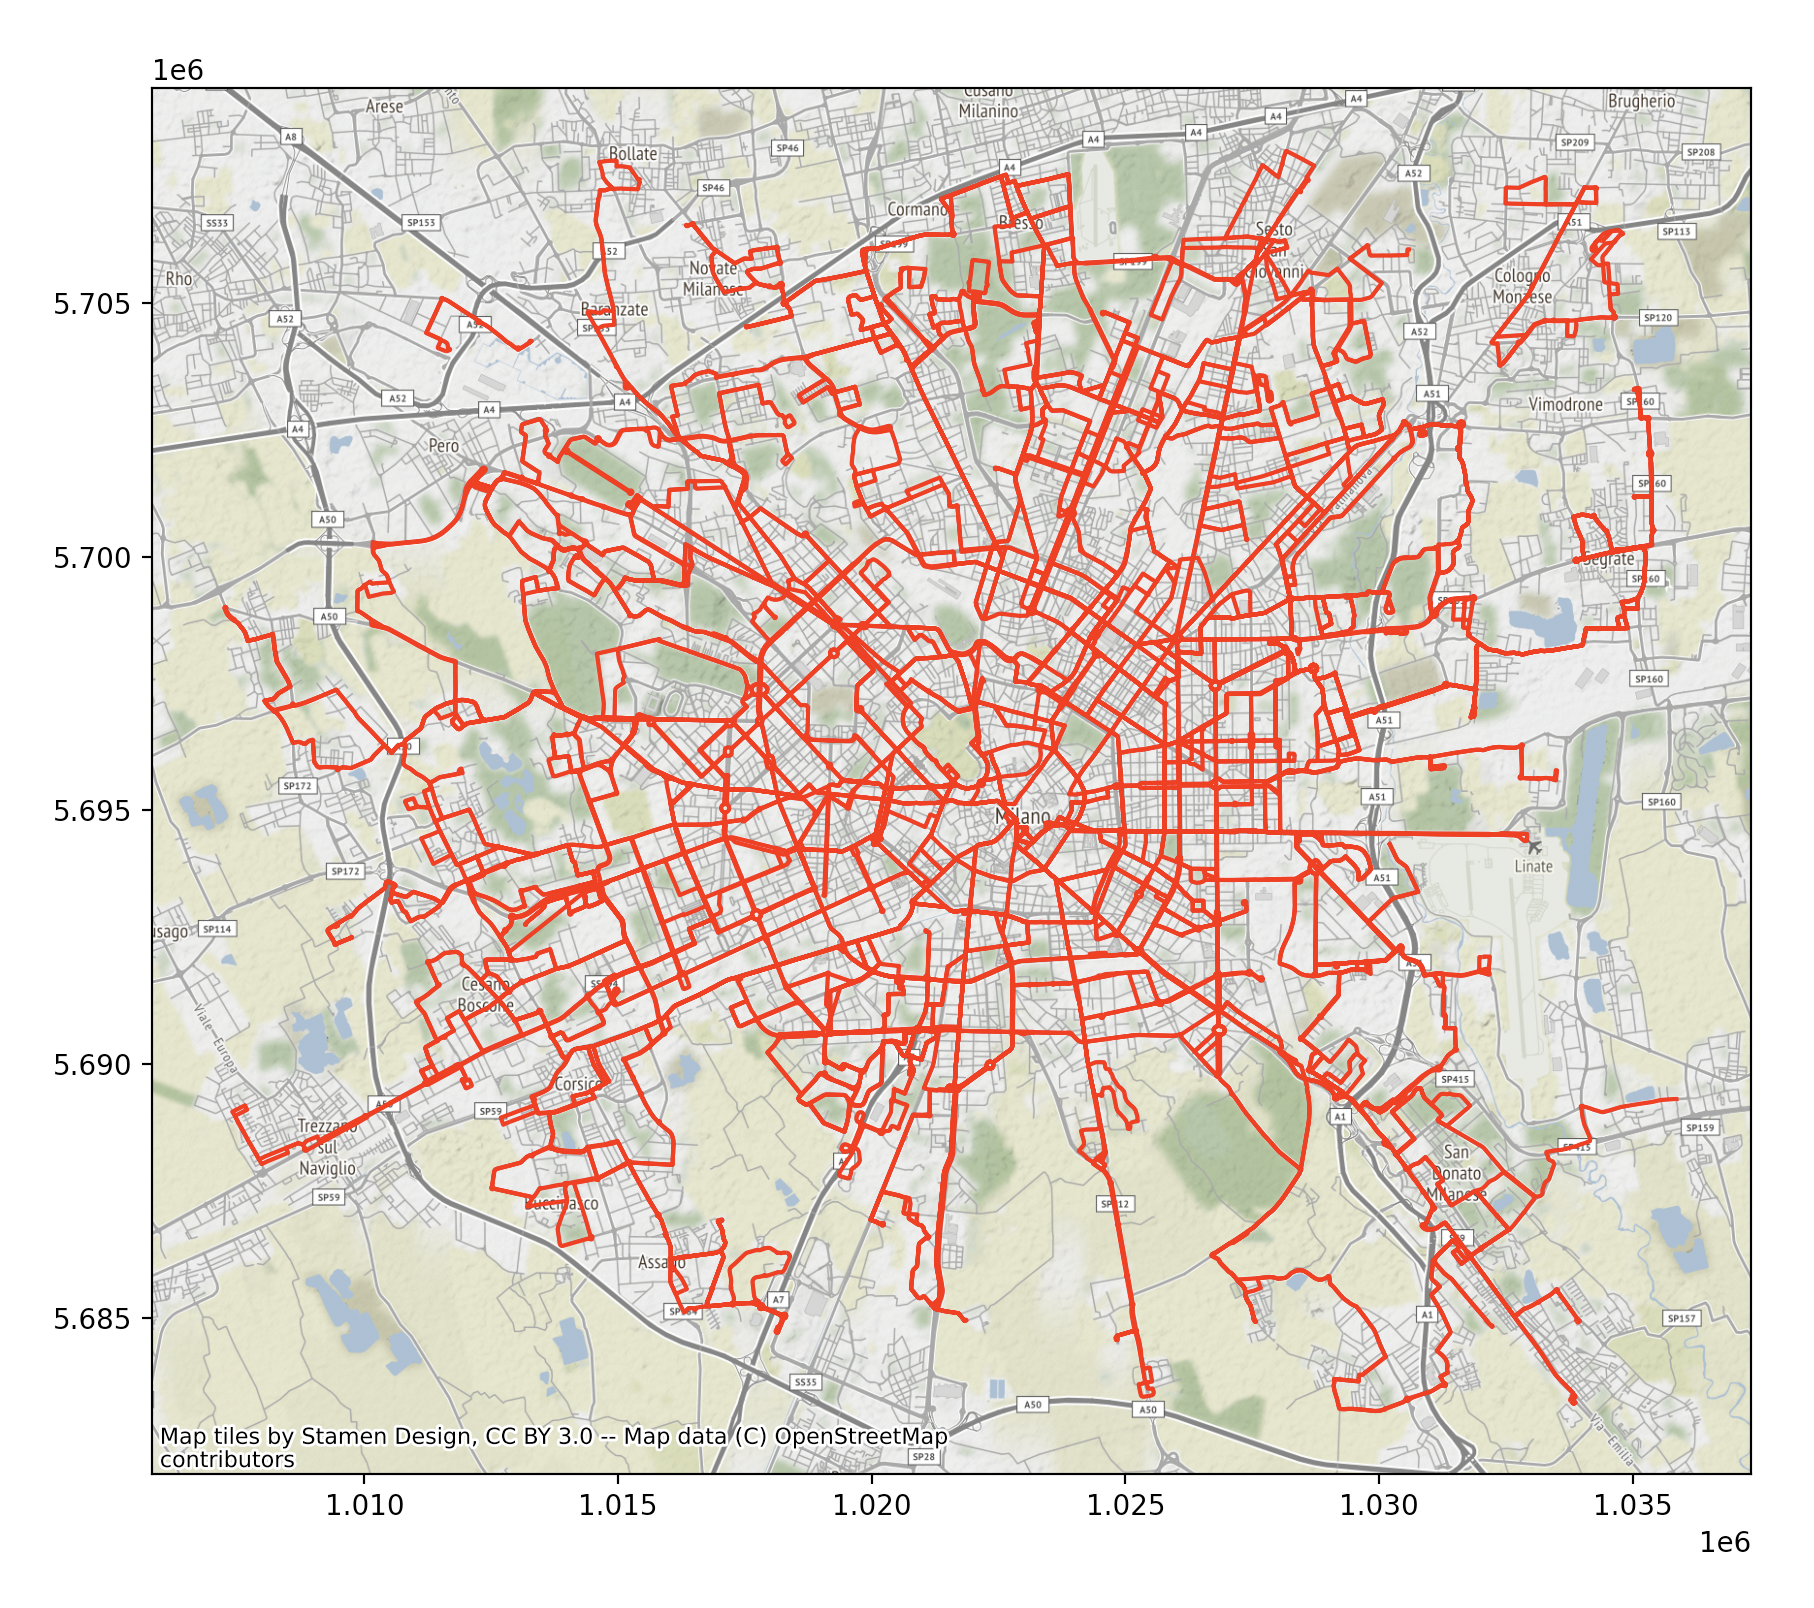
\includegraphics[width=\linewidth]{../src/atm/mappa_2.png}
    \caption{Linee Autobus e Tram a Milano}
    \label{fig:geo_trasporti}
\end{figure}

Se a questi ultimi vengono sovrapposti i dati sugli incidenti, 
si pu\'o notare che la maggior parte dei luoghi con alta concentrazione di incidenti sono 
attraversati da linee di autobus. Nel caso di Corso Ventidue Marzo, si ha anche una linea di tram.
%...
\subsection{Il Pav\'e influisce sull'incidentalità?} Spesso le linee di tram coincidono con
strade in pav\'e
%...
Servirebbe una mappa delle strade in pave a Milano..

% fine della subsection
Dalla sovrapposizione delle mappe, si pu\'o notare anche che, alcune strade con alta incidentalità 
sono parallele a linee di autobus. Un esempio \'e quello di zona Navigli, 
dove le vie interessate sono

\begin{figure}[!ht]
    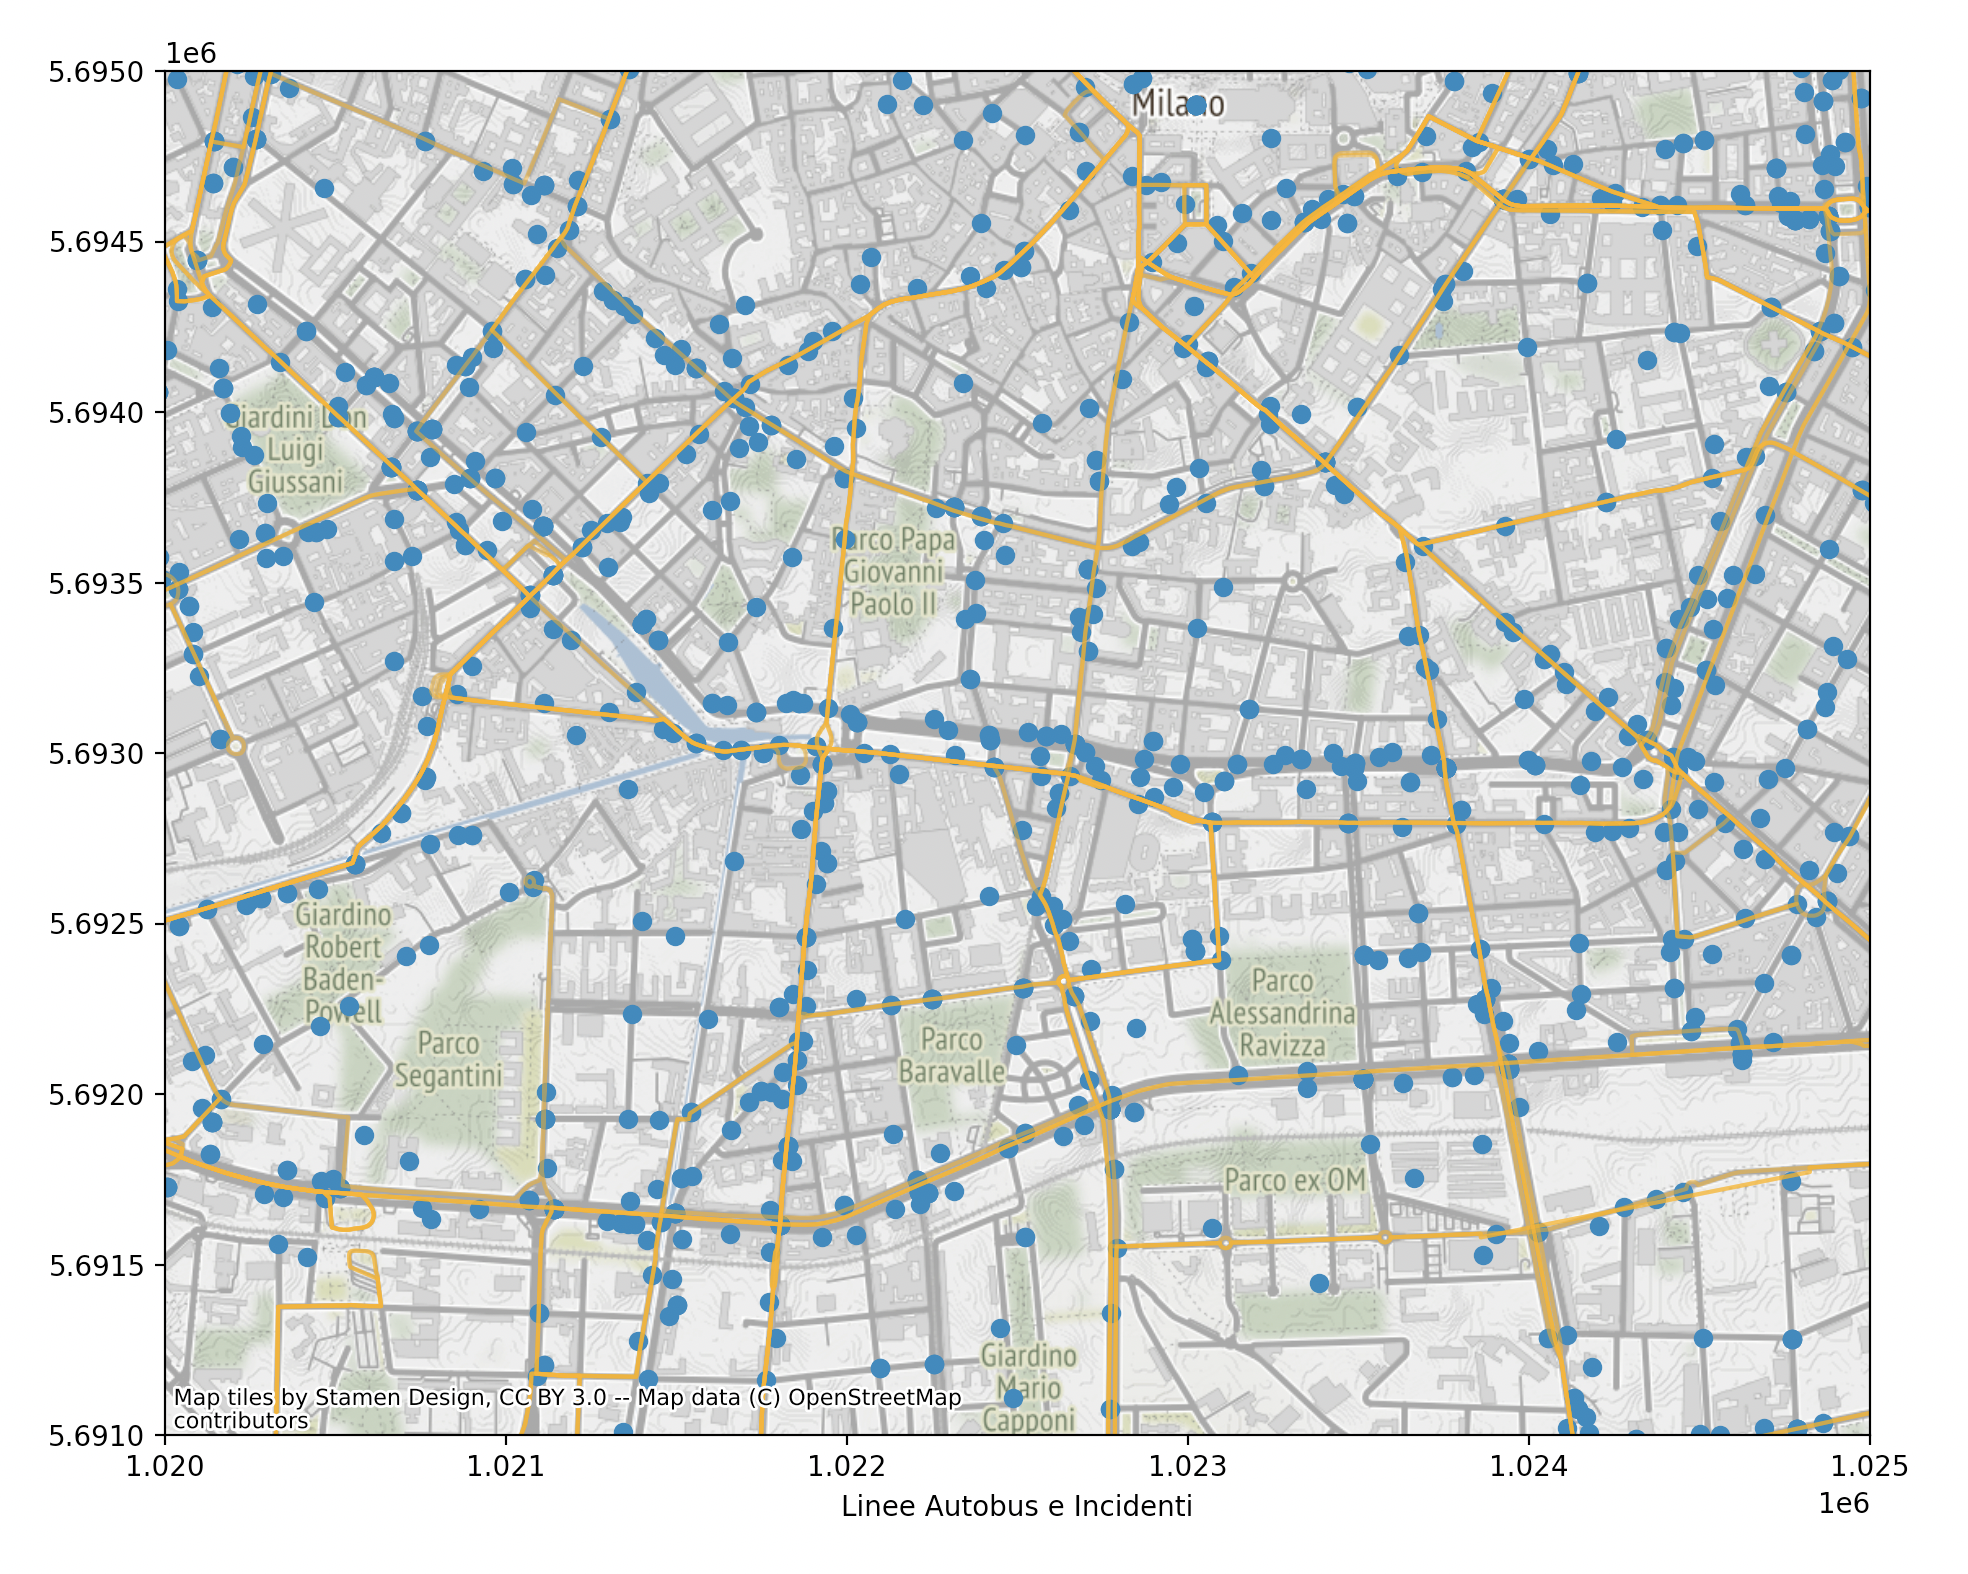
\includegraphics[width=\linewidth]{../src/atm/navigli.png}
    \caption{Linee Autobus e Tram a Milano}
    \label{fig:geo_trasporti}
\end{figure}

Anche vicino a corso Ventidue Marzo si pu\'o notare lo stesso fenomeno, tra le vie

\begin{figure}[!ht]
    \includegraphics[width=\linewidth]{../src/atm/22_marzo.png}
    \caption{Linee Autobus e Tram a Milano}
    \label{fig:geo_trasporti}
\end{figure}



\section{Incidenti e Piste  Ciclabili}

\section{Incidenti e Autovelox}

\section{Incidenti e Meteo}

%%%%%%%%%%%%%%%%%%%%%%%%%%%%%%%%%%%%%%%%%%%%%%%%%%%%%%
\chapter{Dati su Incidenti}
%%%%%%%%%%%%%%%%%%%%%%%%%%%%%%%%%%%%%%%%%%%%%%%%%%%%%%
\chapter{Dati su Meteo}

\bibliographystyle{plain}
\bibliography{Biblio}
%\addcontentsline{toc}{chapter}{Bibliografia}

\end{document}
